%------------------------------------------------
\chapter{\textbf{Introdução}}\label{Introducao}
%---------------------------------------------------------

\section{Relevância e motivação}
A ideia de criar um robô capaz de resolver labirinto surgiu por volta de 1950, construído por Claude Elwood Shannon, sendo que ele que construiu e apresentou pela primeira vez o labirinto original \apud[p. -7]{shannon:2012}{BORGES:2013}. O Micromouse, desde o início, foi planejado para ser um pequeno robô autônomo para percorrer um labirinto. Somente na década de 1970 que iniciou-se a primeira competição, quando o desempenho de vários robôs foi testado para mesma configuração de labirinto \cite{5658360}.

Segundo \citeonline{6734188}, estudantes de engenharia em geral (Elétrica, Computação, Mecânica, entre outros) se empenharam em participar destes campeonatos, uma vez que necessitam-se de pessoas competentes em programação, design de placas, projetos de \textit{hardware}, entre outros. Nos países da Europa (Reino Unido, Portugal), Estados Unidos, Singapura e Japão estas competições são bastantes populares com tais estudantes \cite{6734188}. O estudante de engenharia elétrica aprende, ao longo dos períodos, várias disciplinas, e acaba sendo desestimulado ao se deparar com a falta de prática, ou seja, o que está sendo aprendido em sala de aula às vezes não se acha aplicação útil. Às vezes os alunos preferem aulas mais interativas e querem saber por que o material fornecido na sala de aula é útil em sua carreira. O Micromouse contém a motivação interessante, uma vez que, segundo \citeonline{utad}, o projeto tem caráter multidisciplinar. O estudante aprende a importância de trabalhar com estudantes de outras concentrações de engenharia, o que lhe permite experimentar como uma carreira em futuro trabalho como engenheiro, servindo como experiência em coordenar projetos \cite{remendo1}. 

Portanto, a maior motivação de utilizar a modalidade robótica Micromouse é o seu caráter multidisciplinar da Engenharia Elétrica. Considerada ferramenta de estímulo ao ensino e aprendizado, segundo \citeonline{utad,7344200}, o projeto Micromouse é considerado mais que uma ferramenta para motivar o interesse em alunos na Automação e Controle por promover competências consideradas importantes para estas áreas do conhecimento. \citeonline {remendo1} acrescentaram também que o mini robô móvel autônomo, Micromouse, é ideal para o estudante expandir seus conhecimentos em diversas áreas correlatas, além de relacionar trabalho em equipe.

\section{Descrição do trabalho}
O trabalho desenvolvido consistiu na implementação de algoritmo de resolução de labirinto \emph{Flood Fill} e de controle de trajetórias em Micromouse, com objetivo de penetrar-se em qualquer labirinto real de quase $9 m^2$ de área. A divisão da construção deste projeto será listado a seguir, e, brevemente, comentados:

\begin{enumerate}[leftmargin=2cm,label=\alph*)]
	\item \textit{hardware}: o chassi da plataforma robótica é uma placa de circuito impresso. Além de acomodar toda a parte elétrica com circuito SMD, comporta-se também os motores e sensores. É responsável por movimentar-se fisicamente pelo labirinto de forma inteligente;
	\item algoritmo: responsável por guardar na memória do robô as informações das células e o caminho otimizado, decidir e indicar a orientação da trajetória para a célula seguinte;
	\item controle: esta parte projeta o controle digital para os motores DC, de modo que as velocidades linear e angular sigam as referências pré-estabelecidas pelos perfis de curvas de velocidade.
\end{enumerate}


\section{Revisão da literatura}
Esta seção apresenta uma breve revisão de pontos importantes para a compreensão do trabalho realizado. São tratados, de forma superficial, a história do Micromouse, as regras da competição, a compreensão física e lógica do algoritmo de resolução \emph{Flood Fill}, e o \textit{hardware} do robô. No fim, é apresentado o diagrama do sistema fechado do sistema rodas-\textit{encoder}.

\subsection{História do Micromouse}
Micromouse é uma competição antiga, iniciada na década de 1970. Hoje existem várias competições da modalidade em todo o mundo \cite{5658360}. A competição envolve robôs móveis autônomos para resolver um labirinto composto de 16x16 células de 180 mm de largura, cada. A padronização da competição foi introduzida pela revista do \emph{IEEE Spectrum} em 1977. O robô tem um tempo limitado para resolver um labirinto composto de 256 células, cuja configuração é estabelecida no início da competição \cite{5658360}.

Há mais de 30 anos, Donald Christiansen, chefe da revista \emph{IEEE Spectrum} à época, desafiou os seus leitores a projetar e construir um Micromouse para resolver labirinto. O robô teria sua própria lógica e memória autônomas e exploraria o labirinto que os próprios engenheiros editores do \emph{Spectrum} desenhariam. A configuração do labirinto seria mantida em segredo até o momento da competição. Cada Micromouse teria a oportunidade de investigar o labirinto nas corridas de teste, aprender com seus erros e, assim, poder melhorar seu tempo na corrida. Ele chamou o evento de \emph{Amazing MicroMouse Maze Contest}. Cinco competidores se inscreveram, mas apenas dois atravessaram o labirinto. No entanto, em 1979, quinze Micromouses, dentre os quais o quarto colocado \emph{Moonlight Special}, Figura \ref{fig:MM}, competiram com sucesso nas finais do \emph{Spectrum} em \emph{1979 National Computer Conference} \cite{Christian:2014}.

\begin{figure}[!htb]
	\caption{\label{fig:MM}Robô \emph{Moonlight Special} ficou em quarto lugar no campeonato de 1979, na cidade de Nova York.}
	\begin{center}
		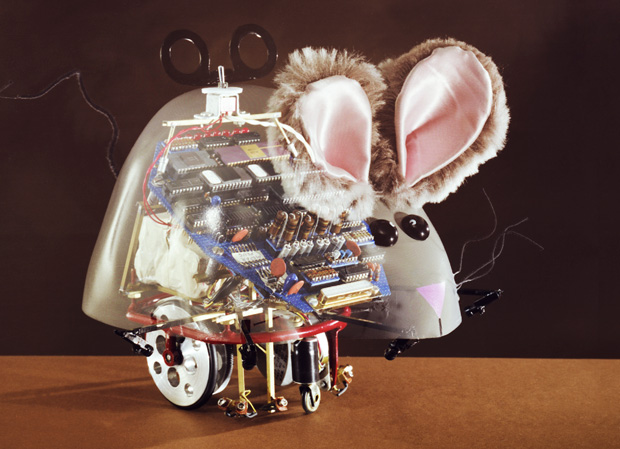
\includegraphics[width=0.6\linewidth]{mm1979.jpeg}
	\end{center}
	\centering
	\small Fonte: adaptado de \citeonline{Christian:2014}
\end{figure}

\begin{citacao}

As finais foram cobertas pela televisão CBS, NBC e ABC e foram relatadas nos noticiários noturnos de Walter Cronkite, John Chancellor e David Brinkley. Recortes de imprensa empilhados de uma ampla gama de jornais, do \emph{International Herald Tribune} ao \emph{Booneville Daily News}, do Missouri. Um Micromouse vencedor foi retratado na primeira página do \emph{The Wall Street Journal} \cite[p. -8]{Christian:2014}.
\end{citacao}

Após alguns anos, o evento tornou-se mundial. Em 1980, a primeira competição europeia foi realizada em Londres, seguida de um ano depois em Paris. O Japão anunciou o primeiro \emph{World Micromouse Contest}, em 1985. \citeonline{Christian:2014} foi convidado a julgar a primeira competição Micromouse em Singapura, em 1987. Neste mesmo ano, o Instituto de Engenharia e Tecnologia organizou uma competição internacional em Londres \cite{Christian:2014}.

Os Micromouses pioneiros eram desengonçados em aparência. Os centros de gravidade eram elevados, com pouca estabilidade. Alguns eram tão altos que tombavam nas curvas. Outros se pareciam mais com \emph{aves} que ratos. Segundo \citeonline{Christian:2014}, \emph{Monty Mouse}, da Grã-Bretanha, parecia um sanduíche de alumínio sobre rodas. As regras da competição da época previam limites de largura e altura além das larguras das células \cite{Christian:2014}.

À medida que a tecnologia avançou, os robôs se mordenizaram tornando-se dispositivos compactados com tecnologia \emph{SMD}, alta densidade de integração que aliado a avanços na tecnologia de construção, tornou os robôs mais compactos e velozes \cite{Christian:2014}. Os avanços nas teorias de controle conferiram maiores capacidades de movimento ao robôs, como por exemplo o movimento controlado em diagonais ao invés de zigue-zague em células quadradas de 180 mm de largura.

Hoje estima-se que são realizados cerca de 100 concursos todo ano. Muitos são patrocinados por universidades e por regiões do IEEE. No Japão, em março de 2014, foi realizada a $35^a$ edição do concurso \emph{All-Japan Micromouse Robot}. Outras competições tradicionais continuam em Mumbai e em Birmingham, Inglaterra \cite{Christian:2014}.

%\subsection{Algorimto de implementação das regras da competição Micromouse}

Considerando as características acima, no Japão, a competição avançou de tal maneira que uma modalidade de labirinto de 32x32 células foi introduzida \cite{6734188}. Na Figura {\ref{fig:japao}}, é mostrada a competição naquele país.


\begin{figure}[!htb]
	\caption{\label{fig:japao}Torneio internacional Micromouse \textit{half-size} no Japão}
	\begin{center}
		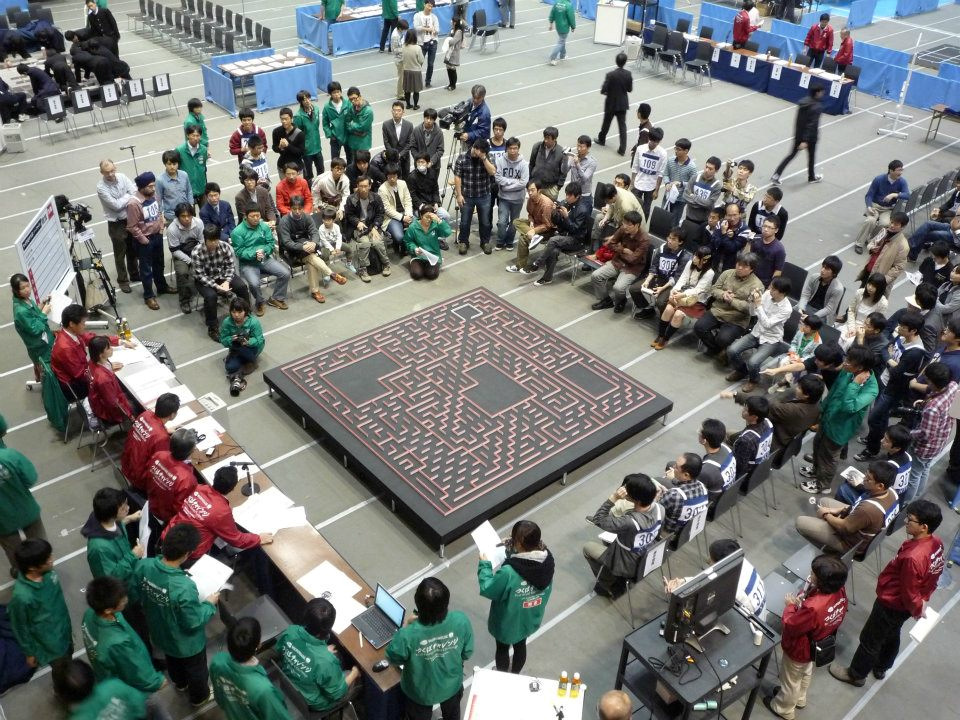
\includegraphics[width=0.6\linewidth]{japao.png}
	\end{center}
	\centering
	\small Fonte: adaptado de \citeonline{6734188}
\end{figure}

\subsection{As regras da competição Micromouse}
A função básica do Micromouse é sair de um dos cantos do labirinto de 16x16 células, de 324 cm$^2$ cada, e chegar ao centro do mesmo. Isto se chama corrida. É contado este tempo. O tempo da corrida do centro do labirinto à célula de partida é desconsiderado. O Micromouse é pontuado de acordo com três parâmetros: velocidade, eficiência em resolver labirinto, e confiabilidade do Micromouse \cite{5658360}.

Além disso, existe um tempo de conhecimento do labirinto para a primeira \emph{corrida}. Em algumas modalidades, Micromouse tem até 15 minutos para fechá-la. Dentro da janela de tempo o Micromouse poderá tentar várias vezes a corrida com o objetivo de diminuir seu tempo \cite{5658360}. A pontuação é baseada tanto na execução mais rápida quanto no tempo total acumulado para todas as corridas. Os donos do Micromouse, de forma alguma, não podem ter nenhum tipo de comunicação com os robôs \cite{Christian:2014}.

O Micromouse deve ser totalmente autônomo. Caso necessite de alguma assistência no meio da corrida, o mesmo é penalizado por \emph{toque}. O Micromouse deve apresentar as seguintes características para resolver com eficiência o labirinto \cite{7344099}: 

\begin{enumerate}[leftmargin=2cm,label=\alph*)]
\item estabilidade Mecânica e Elétrica;
\item velocidade mecânica e de processamento de informação;
\item precisão nos movimentos e sistema de sensores;
\item capacidade de armazenamento eficiente do caminho mais curto;
\item habilidade de resolver, utilizando inteligência computacional, qualquer labirinto regulamentar.
\end{enumerate}


\subsection{Partes do projeto Micromouse}
A seguir são apresentadas as partes primordiais para o projeto de um Micromouse. A harmonia perfeita destes sistemas deixa o mini robô móvel pronto para competições desta modalidade. Eles são responsáveis por dar autonomia ao robô de realizar o trajeto de menor caminho no labirinto de forma inteligente.

\subsubsection{\textit{Hardware}}
A Figura \ref{fig:arranjo} mostra o esquemático geral das conexões dos componentes do Micromouse. Todos os projetos de \textit{hardware} e \emph{design} dos robôs pesquisados na literatura para Micromouse são baseados no arranjo mostrado. Basicamente, em geral, um robô possui microcontrolador, sensores de distância, \emph{encoders}, minimotores de corrente contínua, rodas e bateria para alimentação. O cerebro do robo, o microcontrolador, será capaz de verificar obstáculos à frente com os sensores de distância, tomar decisões e atuar ajustando as velocidades dos motores. A autonomia é garantida pela bateria. Análogo ao sistema humano, o cerebro processa as informações vistas pelos sensores (olhos), processa-as e toma alguma atitude (motores). Então, o robô recebe informações dos sensores e processa-as de forma a comandar corretamente os motores \cite{yadav:2012}.

\begin{figure}[!htb]
	\caption{\label{fig:arranjo}Arranjo físico dos componentes principais do Micromouse}
	\begin{center}
		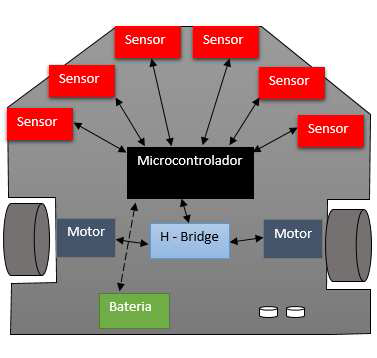
\includegraphics[width=0.4\linewidth]{esquemamicro.png}
	\end{center}
	\centering
	\small Fonte: adaptado de \citeonline{BORGES:2013}
\end{figure}

O Micromouse deve ser uma plataforma autônoma e inteligente, capaz de se locomover em ambientes estreitos de forma rápida. Por isto, segundo \citeonline{nunezdiseno,romo2016diseno}, a tendência de construção seguida para os robôs tentam ser as seguintes:

\begin{enumerate}[leftmargin=2cm,label=\alph*)]
	\item o chassi do robô, normalmente, é a própria placa de circuito impresso, que, por sua vez, tem altura baixa para garantir um centro de gravidade baixo e, consequentemente, maior estabilidade nas curvas;
	\item rodas pneumáticas em cada lado, de forma a aumentar a aderência no piso do labirinto;
	\item pneus de borracha;
	\item motores elétricos, são preferidos os motores DC a motores de passo. No entanto, nos últimos anos os motores sem núcleo ganharam popularidade;
	\item \textit{encoderes} para cada eixo dos motores, com resolução menor que 1 grau por pulso;
	\item sensores de distância, onde os mais populares são os sensores óticos infravermelho (IR);
	\item em geral, se usam quatro ou mais sensores óticos IR em um robô;
	\item baterias Li-PO estão em moda, tendo melhor relação entre a capacidade de carga armazenada, peso e tamanho. São bastante usados em drones por terem estas características;
	\item os microcontroladores mais utilizados são os de 32 bits, com frequência de CPU elevada. Os favoritos são das séries STM32F4 da ST;
	\item sensores como acelerômetros, giroscópios ou bússolas garantem giros precisos de 45, 90 ou 180 graus.
\end{enumerate}

\subsubsection{Algoritmo}
O algoritmo é a parte mais importante para o projeto Micromouse. As direções necessárias para o robô percorrer o menor caminho são obtidas através do algoritmo. Por isso que simpatizantes e fãs deste tipo de robô tentam criar algoritmos mais eficientes a fim de ganhar o campeonato.

A Teoria dos Grafos aparece como uma ferramenta eficiente ao projetar técnicas de resolução de labirinto proficientes. Ao incorporar um procedimento inteligente com os algoritmos de teoria gráfica existentes, alguns algoritmos para Micromouse foram desenvolvidos \cite{5656597}.

O projeto proposto do algoritmo tem como objetivo resolver qualquer labirinto desconhecido, além de ter características otimizadas de consumo de memória, uma vez que circuitos embarcados não possuem grandes quantidades de \emph{RAM}.

Ao buscar referências bibliográficas e arquivos que contenham tais algoritmos inteligentes para resolução de labirinto, foi encontrado um simulador com vários algoritmos já implementados. No \emph{Micro Mouse Maze Editor and Simulator} \cite{solver:2013}, uma ferramenta em Java que mostra como o robô se comporta em diversos labirintos - inclusive alguns já foram labirinto oficial de competição, são encontrados quatro algoritmos. São eles:

\begin{enumerate}[leftmargin=2cm,label=\alph*)]
\item \textbf{Left Wall Follower}: seguidor de paredes à esquerda;
\item \textbf{Right Wall Follower}: seguidor de paredes à direita;
\item \textbf{Treumax}: algoritmo força bruta - visita todas as células do labirinto;
\item \textbf{Flood Fill}: o mais utilizado - simples e eficiente para este tipo de competição.
\end{enumerate}

Os seguidores de parede são os algoritmos mais simples. Pelo fato de existir vários caminhos, ele segue somente o caminho que foi programado, seja à esquerda ou à direita. Segundo \citeonline{remendo3}, algoritmos deste naipe não conseguem lograr êxito em labirintos complexos.

\begin{citacao}

O seguidor de parede é das regras mais conhecidas, também conhecida como a regra da mão esquerda ou direita. Se o labirinto é simplesmente conexo, isto é,
todas as suas paredes estão ligadas entre si ou com limite exterior do labirinto, o algoritmo processa-se mantendo uma mão em contato com uma das paredes do labirinto, onde o jogador está a garantir que não se perde e vai chegar ao centro caso haja uma ligação da parede exterior ao centro. Caso contrário, vai voltar para a entrada após percorrido os corredores do labirinto. Se as paredes estão ligadas, o Micromouse pode ser enganado e fazer um loop ou círculo, não chegando assim ao objetivo. \apud[p. -21--22]{mishabande:2008}{BORGES:2013}

\end{citacao}

O algoritmo Tremaux, na literatura conhecido como \emph{DFS - Depth Firse Search Algorithm}, é um algoritmo que é eficaz, pois resolve muito bem o labirinto, mas o inconveniente dele é o fato de ele percorrer todas as células do labirinto \cite{yadav:2012}. Como o próprio nome sugere, é um algoritmo de pesquisa profunda. É também considerado um algoritmo de Teoria dos Grafos, como o \emph{Flood Fill}. 

No DFS, a partir da raiz do Grafo, o robô desbrava o labirinto até encontrar um beco sem saída, ou seja, até a região mais profunda da árvore ele tenta seguir. Algoritmos começam a procurar a partir de um vértice específico e, em seguida, navega no grafo, ramificando os vértices correspondentes até chegar ao ponto final ou de destino. Este algoritmo de busca pode ser eficientemente usado na resolução de labirintos Micromouse. 

O labirinto inteiro é mapeado como um gráfo onde os nós ou vértices são considerados células de labirinto. Começando a corrida da célula inicial à célula destino, os robôs visitam todas as células, visitando cada entrada aberta das células uma vez em cada direção. Os robôs continuam a pesquisar as células até chegarem à célula de destino. Em vez de marcar cada célula, ele acompanha as paredes celulares. Na corrida inicial, todas as portas da célula original são desmarcadas. 

\begin{citacao}
O algoritmo Trémaux, inventada por Charles Trémaux, é um método eficiente para encontrar a saída de um labirinto que requer o desenho de linhas no chão para marcar um caminho e, é garantido que funcione para todos os labirintos que têm passagens bem definidas. Cada célula do caminho terá um estado de não visitado, marcado uma vez ou marcado duas vezes. Cada vez que um sentido é escolhido, é marcado pelo desenho de uma linha no chão. No início é escolhida uma direção aleatória, caso haja mais do que um. Ao chegar a um cruzamento que não foi visto antes, ou seja sem marcas, escolhe-se uma direção aleatória marcando o caminho. Ao chegar a um cruzamento marcado e se o caminho atual é marcado apenas uma vez, de seguida, vira-se e caminha de volta marcando o caminho uma segunda vez. Se este não é o caso, escolhe a direção com o menor número de marcas. Quando finalmente chegar ao centro, os caminhos marcados exatamente uma vez vão indicar um caminho direto de volta para o início. Se não houver saída, este método irá levá-lo de volta ao começo, sendo que neste caso, cada caminho estará marcado exatamente duas vezes, uma vez em cada direção \apud[p. -22]{Snapp:2010}{BORGES:2013}.

\end{citacao}

O trabalho de \citeonline{5656597} realizou uma comparação entre Tremaux e \emph{Flood Fill}, dois algoritmos surgidos a partir da Teoria dos Grafos, onde mostrou a vantagem do algoritmo de imundação em dois dos três labirintos em descobrir o melhor caminho, explicando o motivo de os competidores preferirem o \emph{Flood Fill} por ele ter a característica de poder encontrar o menor caminho atravessando o número mínimo de células. Afirma-se também que tanto o Tremaux quanto o \emph{Flood Fill} requer grande poder de processamento. O espaço de memória necessário também é muito alto em \emph{Flood Fill}.


A ideia do \emph{Flood Fill} é simples. O \emph{Flood Fill} é um algoritmo que cria uma matriz pré-programada com as dimensões do labirinto, sendo que os números são colocados de uma forma que o labirinto se pareça com um redemoinho, o início tem a numeração mais alta, e o final (chegada) é numerado com zero. O algoritmo somente tenta distribuir as distâncias para cada célula indicando o número de passos para o destino. 

Quando a configuração do labirinto é desconhecido, o mesmo tenta seguir um \emph{atalho} considerando-o como se não existissem paredes, ou seja, sempre tenta seguir um percurso otimista quando não há informações suficientemente. Se existe um caminho mais curto do que o feito, ele já tentou passá-lo. No entanto, às vezes o percurso o leva a caminhos mais longos que o ótimo por ele ter se enganado \emph{nestes caminhos curtos}, e paredes descobertas pelos sensores fazem com que o caminho escolhido na verdade não é o ótimo \cite{5578409}. A ideia desse algoritmo é percorrer as células do maior para o menor valor, uma vez que cada célula tem a distância para o destino \cite{remendo3}.

Dos algoritmos apresentados, segundo \citeonline{utad}, o mais utilizado e um dos mais eficientes é o \textit{Flood Fill} clássico. Ele é baseado em tornar a superfície do tablado em \emph{relevo}, dando números para cada célula. A partir disso, o robô tende a descer esta \emph{superfície} até o ponto mais baixo, em forma de redemoinhos, como faz a água no rio em seu curso natural. O destino sempre tem a numeração 0; uma célula com valor 1 está a um passo do alvo. Se tiver valor 4, está a quatro passos para o destino \cite{utad}.

Já \citeonline{6332345} modificou o algoritmo \emph{Flood Fill} para ter melhor performance do que o tradicional. Segundo ele, o algoritmo \emph{Flood Fill Expected Toll of Penetrating}, assim designado, ele já possui uma inteligência a mais. Ele tenta prever se nas próximas células desconhecidas se há possibilidade de ter uma possível parede, e assim, ele não terá que ir até a célula para verificar isso (Figura \ref{fig:et}). Esta inteligência reduziu os tempos de curvas e números de visitas de células do labirinto \cite{6332345}. 

\begin{figure}[!htb]
	\caption{\label{fig:et}\emph{Flood Fill Expected Toll} - Com expectiva de penetração}
	\begin{center}
		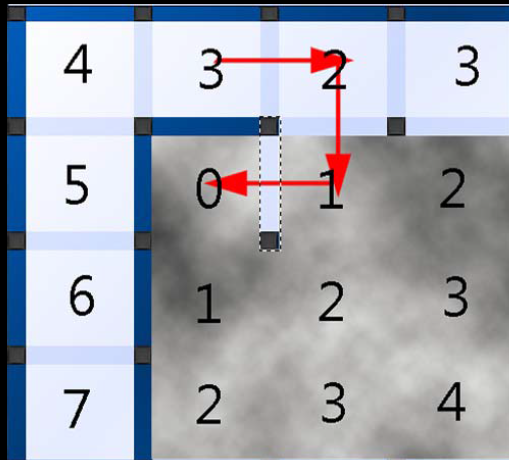
\includegraphics[width=0.6\linewidth]{et.png}
	\end{center}
	\centering
	\small Fonte: adaptado de \citeonline{6332345}
\end{figure}

Porém, nas competições mais atuais, ao realizar corrida, os robôs percorrem em \emph{diagonal} ao invés de realizar contornos em forma de zigue-zague, como mostra a Figura \ref{fig:trajetorias}. Com isto, os robôs evitam perder velocidade nas curvas, o que melhorou e muito o tempo de corrida \cite{6734188}. Este algoritmo é o \emph{diagonal Flood Fill}, considerado melhor, porém não será abordado neste trabalho.

\begin{figure}[!htb]
	\caption[Esquema trajetórias \emph{Flood Fill} clássico e diagonal]{\label{fig:trajetorias}Esquema trajetórias \emph{Flood Fill}}
	\begin{center}
		\subfloat[\emph{Flood Fill} Clássico]{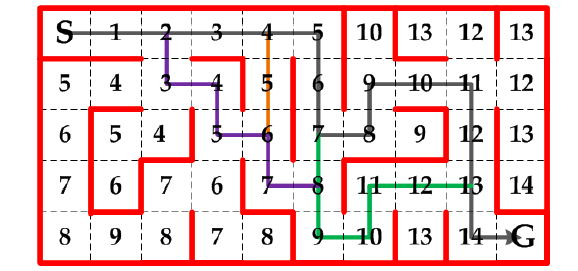
\includegraphics[width=0.4\linewidth]{floodfill.png}}
		\hspace*{0.1\linewidth}
		\subfloat[\emph{Flood Fill} Diagonal]{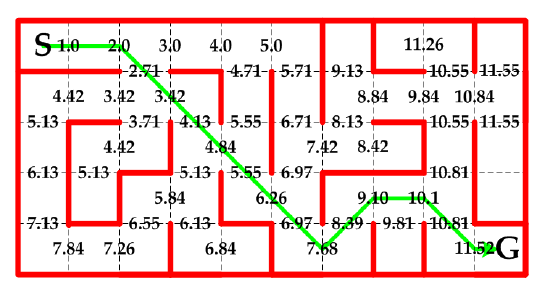
\includegraphics[width=0.4\linewidth]{diagonal.png}}
	\end{center}
	\centering
	\small Fonte: adaptado de \citeonline{6734188}
\end{figure}


\subsubsection{Controle}
Além da eficiência do algoritmo em localizar o melhor caminho, é necessário controle total do seu percurso no labirinto. Ambos devem andar em sintonia perfeita na sua execução.

Como o robô geralmente é móvel diferencial, pode-se prever sua trajetória através das fórmulas cinemáticas (\ref{eq:veloc_v}) e (\ref{eq:veloc_w}), onde $v_R$ é a velocidade da roda direita e $v_L$ é a velocidade da roda esquerda e $L$ é a distância entre as rodas. As velocidades das rodas estão diretamente ligadas com as velocidades linear ($v_C$) e angular ($\omega_C$) global do robô. Então, as informações digitais dos \emph{encoders} são usadas para controlar o movimento da trajetória do Micromouse \cite{6734188}.

\begin{figure}[!htb]
	\caption{\label{fig:curva}Percurso em curva de 90 graus.}
	\begin{center}
		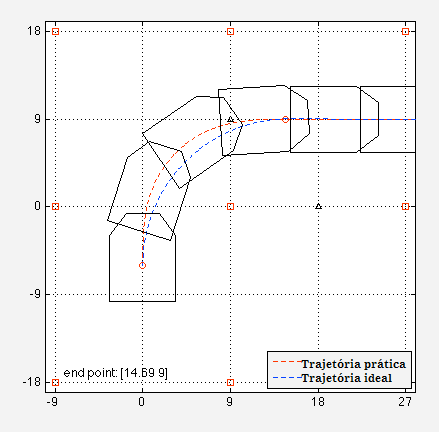
\includegraphics[width=0.7\linewidth]{curva.png}
	\end{center}
	\centering
	\small Fonte: adaptado de \citeonline{6734188}
\end{figure}

\begin{equation}
	\label{eq:veloc_v}
	v_C 	=	(v_R + v_L)/2
\end{equation}

\begin{equation}
	\label{eq:veloc_w}
	\omega_C 	=	(v_R - v_L)/L
\end{equation}

Com o raio da curva é conhecido, e predefinindo valores de velocidade linear, e que o robô realizará uma curva de 90 graus em uma célula, pode-se traçar um perfil de curva. Um exemplo é mostrado na Figura \ref{fig:curva}.

\citeonline{6734188} sugerem criar um controlador digital (Figura \ref{fig:controlador}) com dois \emph{set points}: velocidade linear e angular. Quem os alimenta são os \emph{speed profiles}, que podem ser simulados no \textit{EXCEL} ou \textit{MATLAB}. O controlador será responsável por aplicar as velocidades das rodas de maneira tal que o robô tenha realmente ambas as velocidades do \textit{speed profile}. O sistema será realimentado através das informações dos \emph{encoders} e os controladores {PID} (Proporcional, Integral e Derivativo) darão os \emph{duty cicle} dos sinais {PWM} aos motores de corrente contínua (DC). A Figura \ref{fig:controlador} mostra melhor o esquema de controle.  Assim, o robô obedecerá a trajetória de Figura \ref{fig:curva}.

\begin{figure}[!htb]
	\caption{\label{fig:controlador}Controlador Digital realimentado para robôs autônomos diferenciais}
	\begin{center}
		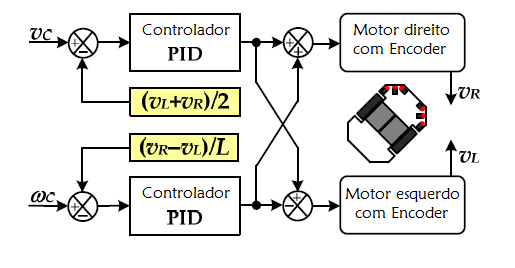
\includegraphics[width=0.9\linewidth]{controlador.png}
	\end{center}
	\centering
	\small Fonte: adaptado de \citeonline{6734188}
\end{figure}


\section{Metodologia}
O estudo realizado consistiu no projeto das três partes necessárias, utilizando como ponto de partida as observações feitas em algoritmos de resolução de labirinto \emph{Flood Fill}, que foi baseado nos trabalhos de \citeonline{remendo3} e \citeonline{6332345}. 

O algoritmo de otimização proposto, implementado em C, utiliza um conjunto de simbolos que permite a análise do percurso de rota do robô no labirinto. Os símbolos são úteis em um processo de depuração de corridas, a fim de validar a eficácia do algoritmo. A seguir são mostrados alguns símbolos básicos essenciais para depurações. Os símbolos \verb+|+ e \verb+---+ significam as paredes nos vértices das células, sendo que o caractere \texttt{+} simboliza as quinas das células. Os números em cada célula significam o número de passos para o destino. Na célula onde o robô se encontra, os símbolos \texttt{V}, \texttt{\^}, \texttt{>} e \texttt{<} indicam o sentido, e o símbolo \texttt{*} nas células mostram onde o robô já visitou. A Figura \ref{fig:simbolos} mostra um exemplo para utilização dos símbolos.

%It is essential for debugging to be able to print out your maze

\begin{figure}[!htb]
	\caption{\label{fig:simbolos}Símbolos utilizados para impressões}
	\begin{center}
		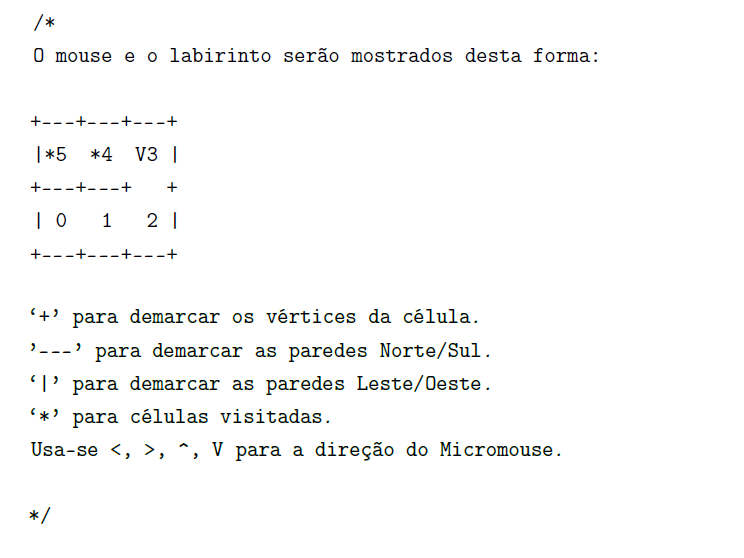
\includegraphics[width=0.9\linewidth]{simbolos.png}
	\end{center}
	\centering
	\small Fonte: autor (2017)
\end{figure}

%\begin{verbatim}
%	+----+----+----+
%	|*  5 *  4 V  3|
%	+----+----+    +
%	|   0    1    2| 
%	+----+----+----+
%\end{verbatim}


Já as constantes do controle PID do robô foram extraídas a partir do \emph{Método do Relé Sequencial}, tendo como prioridade a maximização do tempo de assentamento, visto que quanto mais rápido chegar nas velocidades de referência, a trajetória em curvas se torna próxima à trajetória ideal (Figura \ref{fig:curva}).

O desempenho do controlador para as rodas do Micromouse foi verificado no ambiente Simulink do \textit{MATLAB}. Após a realização da identificação do sistema robô-rodas do Micromouse, através do Método dos Mínimos Quadrados Não Recursivos (MQNR), foi construído um modelo de controle das velocidades das rodas com base no esquema de controle proposto por \citeonline{6734188} e pode-se verificar as trajetórias em curvas e retas ao variar as referências de velocidades linear e angular.

Após a verificação das partes de forma individual, foram realizados testes com todos as partes em conjunto em um labirinto de testes, contruído a partir de placas de MDF, a fim de verificar o comportamento do mini robô em um labirinto real.

\section{Objetivos}
A seguir são apresentados os objetivos desejados com o estudo realizado. É apresentado, inicialmente, o objetivo geral deste trabalho e, em seguida, listam-se objetivos específicos que se desejam alcançar.

\subsection{Objetivo geral}
Estudar, desenvolver, simular e implementar, juntamente com o controle de velocidades, o algoritmo inteligente de resolução de labirinto em mini robô Micromouse. Desenvolver o projeto do mini robô autônomo diferencial Micromouse.

\subsection{Objetivos específicos}
Os objetivos específicos que se deseja alcançar com o trabalho são os seguintes:

\begin{enumerate}[leftmargin=2cm,label=\alph*)]
	\item Aplicar os conhecimentos adquiridos em programação no curso de Engenharia Elétrica para desenvolver algoritmo de resolução de labirinto, na liguagem C, para facilitar a inclusão do mesmo em quaisquer microcontroladores;
	\item Desenvolver o controle digital de velocidade linear e angular de forma que o robô tenha facilidade em andar em linha reta e em curvas.
	\item Tornar o Micromouse autônomo e inteligente o suficiente a descobrir o menor caminho em labirinto desconhecido real.
\end{enumerate}


\section{Estrutura do trabalho}
Este trabalho é estruturado em quatro capítulos, conforme as descrições que seguem:

\begin{enumerate}[leftmargin=2cm,label=\alph*)]
	\item \textbf{Capítulo 01}: introdução acerca do tema tratado, motivação do estudo e contextualização do tema na sociedade atual;
	\item \textbf{Capítulo 02}: neste capítulo são realizadas análises específicas sobre cada uma das partes implementadas e são apresentadas as informações presentes na literatura sobre eles;
	\item \textbf{Capítulo 03}: apresenta as partes projetadas e os resultados observados em suas simulações e em labirinto, bem como observações pertinentes acerca desses resultados;
	\item \textbf{Capítulo 04}: são apresentadas, sucintamente, as principais conclusões observadas no trabalho, além de sugestões para futuros trabalhos nessa linha.
\end{enumerate}